\documentclass{beamer}
\usepackage[utf8]{inputenc}
\usepackage[T1]{fontenc}
\usepackage{lipsum, lmodern}
\usepackage{amsmath,amsthm,amssymb,mathrsfs,mathtools,amsfonts,braket,bm}
\usetheme{Median}
\usepackage{bibentry}
\nobibliography*
\def\description#1{}
\author{Eduardo Gonzalez Lazo }
\title{Streamlining Development with CMake Presets}
\institute{
	\begin{center}
		Italian C++ Community meetup
	\end{center}
}
\date{\today}
\setbeamercovered{transparent}
\def\beamertemplatetransparentcoveredmedium{\setbeamercovered{transparent=65}}
\beamertemplatetransparentcoveredmedium
\begin{document}
\frame{\maketitle}
\description{
	This presentation provides a general overview of creating self-contained and reusable CMake projects, with a focus on introducing and leveraging CMake Presets. While CMake Presets have been available for some time, they remain relatively underutilized by developers. However, their adoption is steadily growing, particularly in modern IDEs and continuous integration (CI) pipelines.%
	The session will demonstrate how combining CMake Presets with a well-structured CMake configuration can streamline the process of building projects that are both self-contained and easy to reuse. Key points for crafting reusable projects, such as creating libraries that can be seamlessly imported using find_package and other best practices, will also be discussed.
}

\begin{frame}{About Me}
	\begin{center}
	Eduardo Gonzalez Lazo 

	\href{mailto:eduardo.gonzalez@amarulasolutions.com}{eduardo.gonzalez@amarulasolutions.com}

	\vspace{1cm}
	Embedded Linux consultant \& developer at 

	\textbf{\href{https://www.amarulasolutions.com/}{Amarula Solutions}}

	\vspace{1cm}
	Open Source enthusiast \& Developer advocate
	\end{center}
\end{frame}
\section{Introduction}%
\begin{frame}[fragile]{Why we love CMake}%
	\vspace{1cm}
	\begin{block}{Cross-Platform}%
		\begin{itemize}%\small
			\item Works on Windows, Linux, macOS ...%
			% and can produce binaries also for IOS, Android, WebAssembly, etc.
			\item Supports multiple compilers%
			\item Generates native build files for various tools
			\item Packaging, Testing%
			% We can say CMake is the de-facto standard for building C++ code.
			% It provide a set of tools that allow to package the code, test it, and build it.
			% With a simple syntax, from your preferred desktop distribution to a variety of target platforms.
		\end{itemize}%
	\end{block}%
	\begin{block}{Modular, Reusable and Scalable}%
		\begin{itemize}%\small
			\item Modern CMake and its targets%
			% CMake has the concept of targets where one can define its properties, dependencies, include headers, etc.
			% This allows to create a modularized project that can be reused in other projects.
			\item Consume the reusable modules%
			\begin{itemize}
				\item \texttt{add\_subdirectory()}
				\item \texttt{FetchContent...}
				\item \texttt{find\_package()}
				% add_subdirectory and fetchContent are normally used Download and build source code while find_package
				% is used to consume a `library` that is already compiled in the system(like the SDK of the library).
				% But the two first can be also used to consume a `library`' that is already compiled.
				% because find_package only search for a cmake file that creates imported targets from compiled 
				% libraries and headers on the system.
				% A file that creates imported targets can also be loaded/configured by add_subdirectory or FetchContent.
			\end{itemize}%	
		\end{itemize}%	
	\end{block}%
	% From a developer perspective you have everything with CMake and C++.
	% You develop a C++ library that in principle will work in many platforms.
	% With CMake you can create a reusable project that can build, test, and package the library in a cross-platform way.
	% And with CMake Presets you can share the different configurations of the project with other developers.
	% So one has the opportunity to create a project that is easy to use, easy to maintain, and easy to share.
	% In this times with AI anyone can write C++ code, but not everyone can create a project that is easy to use and maintain. 
\end{frame}
\begin{frame}[fragile]{Readme.md}\small%
	\vspace{0.2cm}
	\begin{center}
	\begin{block}{Reusable, self contained CMake projects}
		% Creating a reusable self contained CMake project is a broad topic and could be complicated
		% if we care about cross-platform compatibility. When i say self-contained I could be also implying well-defined.
		% Well defined, in the sense that is clear how to use it.  
		% So in this talk I will only explain how to create the exports of the targets and the logic behind 
		% for your targets become available with a call to find_package.
		\begin{itemize}
			\item \texttt{find\_package}: Create exports for the targets
				% This is a very important point. When creating a library that is going to be used by other projects
				\begin{itemize}
					\item Declare/Export target dependencies
				% As a consumer project we can link to a library but we do not have to link to the library
				% public dependencies. So the library is self-contained.
				\end{itemize}
		\end{itemize}
	\end{block}
	\vspace{0.4cm}
	\begin{block}{CMake Presets}
			\begin{itemize}
				\item General overview
					% The structure of the files, the common fields, and the different types of presets and its purpose. 
				\item Showcase its support/adoption
					% In modern IDEs and in CI pipelines.
				\item Role in creating self-contained and reusable projects
					% We will see how these are also enclosed in the topic of creating
					% a reusable self-contained CMake project.
					% and improving developer workflow.
			\end{itemize}
	\end{block}
	\end{center}
\end{frame}

\begin{frame}[fragile]{Modern CMake and its targets}%
	\vspace{1cm}
	\lstinputlisting[firstline=30, lastline=36]{../CMakeLists.txt}
	\lstinputlisting[firstline=50, lastline=52]{../CMakeLists.txt}
	\begin{block}{\small Consume the module/targets}
		\begin{itemize}\small%
			\item \texttt{add\_subdirectory()}%
			\item \texttt{FetchContent\_MakeAvailable()}%
		\end{itemize}
	\end{block}
\end{frame}

\begin{frame}[fragile]{Export the targets}%
	\vspace{1cm}
	\roundedBlock{Install interface}{
		\lstinputlisting[firstline=99, lastline=103]{../CMakeLists.txt}
	}{}{0.9\textwidth}
	% Here we have the install EXPORT command. This will create a export file called 
	% ProjectName-config.cmake with the targets that were exported and hopefully installed by this project.
	% Simply it creates imported targets using the already installed targets.
	\roundedBlock{Build interface}{
		\lstinputlisting[firstline=122, lastline=125]{../CMakeLists.txt}
	}{}{0.9\textwidth}
	% The export EXPORT command. Do the same that the previous install command 
	% but it will use the targets from the build directory.
	% There are other ways to create the export file, but these are the most common.
	% this command is very nice because one does not have to install the project to be able to use find_package 
	% to consume it. 
	% But it is very likely one will get the error that there are targets that are not in any export set.
	% from the dependencies. In this project i use Qt and Boost using find_package and in this case the targets
	% Qt6::Core and Boost::program_options are in a export set.
	% But if I use the Qt/Boost targets by using add_subdirectory or FetchContent these targets will not be in any export set.
	% So the consumer of this project will get an error when trying to use the exported targets.
	\begin{block}{\small Consume the module/targets}
		\begin{itemize}\small%
			\item \texttt{find\_package()}%
		\end{itemize}
	\end{block}
\end{frame}

\begin{frame}[fragile]{Associate targets with the export and install}%
	\vspace{1cm}
	\lstinputlisting[firstline=43, lastline=47]{../CMakeLists.txt}
	\lstinputlisting[firstline=38, lastline=41]{../CMakeLists.txt}
	\begin{block}{\small Modular Install}
		\begin{itemize}\small%
			\item Group by \texttt{COMPONENT}s%
			\item Associate targets with export
			\item Used by CPack to create binary installers
		\end{itemize}
	\end{block}
	% We have the CMake install command that allows to install/add to the package the different
	% targets and files. It allows to set the destination and group these in components.
	% These instructions are used by CPack to create the binary installers with different generators.
	% Generators like NSIS, DEB, TAR, etc.
	% In this example we add the library target to the package and the export file.
	% The previous export commands will add the targets to the export file.
	% It use the default install path depending on the type of the library(shared, static, windows, linux).
	% It adds by default the library to a certain component.
	% If the library is a static library will be added to the development component.
	% We also install the headers of the library and add them to the development component.
	% With this we can create package with only the runtime components or with the development components.
	% This decision is made when using the cpack command or as we will see later with the CMake Presets.
\end{frame}

\begin{frame}[fragile]{Define the dependency targets and the version}\small%
	\vspace{1cm}

	\lstinputlisting[firstline=108, lastline=112]{../CMakeLists.txt}
	% Here we have the configure_package_config_file command.
	\only<1>{\roundedBlock{Config.cmake.in}{
		\lstinputlisting[firstline=1, lastline=4]{../Config.cmake.in}
	}{}{0.9\textwidth}
	
				% I have found projects that use `pkg_check_modules`
				% instead of using find_package when doing this.
				% The problem with this is that pkg does not use targets.
				% Then one needs to somehow find and link the library dependencies
				% This clutters the CMake configuration and makes the projects
				% more difficult to maintain and to scale.
				% Ex. If the library removes one of its dependencies it is very probable this
				% dependency stays in the consumer project a long time.
				% If the project is well defined should declare the public dependencies in the exports also,
				% not only declare the targets. So this is a very important point in creating a self contained easy to reuse project.
	
		\begin{center}
			$\downarrow$
		\end{center}
	\lstinputlisting[firstline=32, lastline=33]{../CMakeLists.txt}}
	% Only public dependencies should be declared in the exports.
	% In this case, the library depends on Qt6::Core and Boost::program_options.
	% But the consumer of the CMake export only need to know about the Qt6::Core dependency.
	% because it is the one added to the public interface of the library.
	% When a consumer checks the exports of the library it will see that it depends on Qt6::Core,
	% So this target should be defined before that(it is defined by find_dependency/find_package).
	\only<2->{
	\lstinputlisting[firstline=113, lastline=116]{../CMakeLists.txt}}
	\only<3->{
	\lstinputlisting[firstline=117, lastline=121]{../CMakeLists.txt}}
	\only<4->{
		\begin{block}{\small \texttt{find\_package} will work using}
			\begin{itemize}\small%
				\item Build directory%
				\item CMake installation directory%
				\item CPack installation directory%
			\end{itemize}
		\end{block}
	}
\end{frame}
\begin{frame}[fragile]{Reusing the library}\small%
	\vspace{1cm}

	\lstinputlisting[firstline=14, lastline=22]{../LibraryConsumer/CMakeLists.txt}
	\lstinputlisting[firstline=24, lastline=26]{../LibraryConsumer/CMakeLists.txt}
	\begin{block}{\small Why use \texttt{find\_package()}}
		\begin{itemize}\small%
			\item Make available the targets%
			\item Declare its dependencies%
			% Not need to carry the dependencies of the library in the consumer project.
			% The library/project is well defined.
			\item Unified logic to consume the package%
			% There are no If statements! the way the target is linked is the same if found by find_package or
			% made available by fetchContent.
			% The targets are available if already in the system, if not they will become available by fetchcontent.
			% In this way, we allow the consumer to be self-contained when using our library/project.
			\item Simple logic to create the exports%
			% Creating the export is relatively simple if one already has a CMake Project with the targets.
			% And the exports will work the same if using the build/install/cpack directory.
		\end{itemize}
		% These, will improve the maintainability of the projects. 
	\end{block}
\end{frame}
\bigtemplate{Demo time}{
}
\begin{frame}[fragile]{Configure, build, test, package}\footnotesize%
	\vspace{1.0cm}
	% Now we have a modularized, self-contained CMake project with well-defined targets.
	% Let's use it.
	% This could be a normal workflow for a developer working with a CMake project.
	% We have the configure part where we set the generator, the build type, etc.
	% We add some paths so that find_package can find Qt targets,
	% and set not to build a part of the project maybe because we do not have the dependencies installed.
	% We have the build step, then the developer can also run the tests or package the binary installers.
	% There is no problem with this, it is still mostly cross-platform.
	% But how do we share this flow with new developers?
	% We add this to the README of the project, if the project has many configuration paths
	% this is difficult to maintain.
	% We create scripts to automate this that is also difficult to make it cross-platform.
	% Is there a standardized way to do this, to share the configuration settings of a project or the
	% developer workflow in general?
	\begin{block}{\footnotesize Configure}
			\begin{lstlisting}[language=sh]
				cmake -G Ninja -S . -B build-release -DCMAKE_PREFIX_PATH=/home/amarula/Qt/6.8.0/gcc_64/
				-DBUILD_SERVER=OFF -DCMAKE_BUILD_TYPE=Release -DBUILD_SHARED_LIBS=ON
			\end{lstlisting}
	\end{block}
	\begin{block}{\footnotesize Build}
			\begin{lstlisting}[language=sh]
				cmake --build build-release/ --parallel 4 --target getClientCode
			\end{lstlisting}
	\end{block}
	\begin{block}{\footnotesize Test}
			\begin{lstlisting}[language=sh]
				ctest --stop-on-failure --timeout 10 --test-dir build-release/
			\end{lstlisting}
	\end{block}
	\begin{block}{\footnotesize Package}
			\begin{lstlisting}[language=sh]
				cpack -V -B package -G "IFW;TGZ" --config CPackConfig.cmake
			\end{lstlisting}
	\end{block}
\end{frame}

\bigtemplate{CMake Presets}{
	% Using CMake Presets should be the standardized way to do this.
	% Although they have been available for some time, they remain relatively underutilized by developers.
	% I am normally aware of the last nice features of CMake, but this one I had never hear before.
	% My boss was trying to share the different build configuration with many ways to be configured.
	% And he recommended to check this, and I found it very useful when improving the developers workflow
	% and his interaction with the project.
}

\begin{frame}[fragile]{Configure, build, test, package}\footnotesize%
	\vspace{1.0cm}
	% So all these different steps/commands can use a preset.
 	\begin{block}{\footnotesize Configure}
		\begin{onlyenv}<1>
			\begin{lstlisting}[language=sh]
				cmake -G Ninja -S . -B build-release -DCMAKE_PREFIX_PATH=/home/amarula/Qt/6.8.0/gcc_64/
				-DBUILD_SERVER=OFF -DCMAKE_BUILD_TYPE=Release -DBUILD_SHARED_LIBS=ON
			\end{lstlisting}
		\end{onlyenv}
		\begin{onlyenv}<2->
			\begin{lstlisting}[language=sh]
				cmake --preset user-release
			\end{lstlisting}
		\end{onlyenv}
	\end{block}
	\begin{block}{\footnotesize Build}
		\begin{onlyenv}<1-2>
			\begin{lstlisting}[language=sh]
				cmake --build build-release/ --parallel 4 --target getClientCode
			\end{lstlisting}
		\end{onlyenv}
		\begin{onlyenv}<3->
			\begin{lstlisting}[language=sh]
				cmake --build --preset userGetClientCode
			\end{lstlisting}
		\end{onlyenv}
	\end{block}
	\begin{block}{\footnotesize Test}
		\begin{onlyenv}<1-3>
			\begin{lstlisting}[language=sh]
				ctest --stop-on-failure --timeout 10 --test-dir build-release/
			\end{lstlisting}
		\end{onlyenv}
		\begin{onlyenv}<4->
			\begin{lstlisting}[language=sh]
				ctest --preset user-debug
			\end{lstlisting}
		\end{onlyenv}
	\end{block}
	\begin{block}{\footnotesize Package}
		\begin{onlyenv}<1-4>
			\begin{lstlisting}[language=sh]
				cpack -V -B package -G "IFW;TGZ" --config CPackConfig.cmake
			\end{lstlisting}
		\end{onlyenv}
		\begin{onlyenv}<5->
			\begin{lstlisting}[language=sh]
				cpack --preset user-release
			\end{lstlisting}
		\end{onlyenv}
		\begin{onlyenv}<6->
	\begin{block}{\footnotesize Workflow}
		\begin{lstlisting}[language=sh]
			cpack --workflow --preset user-release
		\end{lstlisting}
	\end{block}
		\end{onlyenv}
	\end{block}
\end{frame}
\begin{frame}[fragile]{CMake Presets}\small%    
	\vspace{1cm}
	\begin{columns}
		\column{0.6\textwidth}
		\begin{itemize}
			\item Configure presets
			\item Build presets
			\item Test presets
			\item Package presets
			\item Workflow presets
		\end{itemize}
		\column{0.3\textwidth}
		\only<2->{
			\begin{block}{Common fields}
			\begin{itemize}\footnotesize
				\item \texttt{name}
				\item \texttt{description}
				\uncover<3->{\item \texttt{hidden}
				\item \texttt{inherits}}
				\uncover<4->{\item \texttt{condition}}
				\uncover<5->{\item \texttt{vendor}}
			\end{itemize}
		\end{block}
		}
	\end{columns}			
	\begin{onlyenv}<2>
		\lstinputlisting[firstline=8, lastline=12]{../CMakePresets.json}
	\end{onlyenv}
	\begin{onlyenv}<3>
		\lstinputlisting[firstline=20, lastline=26]{../CMakePresets.json}
	\end{onlyenv}
	\begin{onlyenv}<4>
		\lstinputlisting[firstline=94, lastline=101]{../CMakePresets.json}
	\end{onlyenv}
	\begin{onlyenv}<5>
		\lstinputlisting[firstline=42, lastline=49]{../CMakeUserPresets.json}
	\end{onlyenv}
			% At the moment of the presentation, these are the supported presets.
			% One has different JSON objects with different required/optional fields.
			% The presets have common fields like name.

			% Apart from that every preset has specific fields for each stage.
			% These are related (as we have seen) to command lines arguments when using cmake for configuring, building
			% or using ctest and cpack commands.
\end{frame}
\begin{frame}[fragile]{CMake Presets}\small%    
	\vspace{1cm}
	\begin{columns}
		\column{0.3\textwidth}
		\begin{itemize}
			\item Configure presets
			\item Build presets
			\item Test presets
			\item Package presets
			\item Workflow presets
		\end{itemize}
		\column{0.5\textwidth}
		
		\begin{block}{Not common fields}
		\begin{itemize}\footnotesize
			\item \texttt{cacheVariables}, \texttt{toolchainFile}
			\item \texttt{targets}, \texttt{configurePreset}
			\item \texttt{outputOnFailure}
			\item \texttt{generators}, \texttt{configFile}
			\item \texttt{steps}
		\end{itemize}
		\end{block}
	\end{columns}
	\vspace{1cm}
	\begin{onlyenv}<1>
		\lstinputlisting[firstline=24, lastline=29]{../CMakePresets.json}
	\end{onlyenv}
	\begin{onlyenv}<2>
		\lstinputlisting[firstline=83, lastline=87]{../CMakePresets.json}
	\end{onlyenv}
	\begin{onlyenv}<3>
		\lstinputlisting[firstline=108, lastline=114]{../CMakePresets.json}
	\end{onlyenv}
	\begin{onlyenv}<4>
		\lstinputlisting[firstline=122, lastline=129]{../CMakePresets.json}
	\end{onlyenv}
\end{frame}
\begin{frame}[fragile]{CMake Presets}\small%    
	\vspace{1cm}
	\begin{block}{Workflow presets}
		A sequence of configure, build, test, and package steps
	\end{block}
	\vspace{1cm}
	\begin{onlyenv}<1>
		\lstinputlisting[firstline=145, lastline=158]{../CMakePresets.json}
	\end{onlyenv}
	\begin{onlyenv}<2>
		\lstinputlisting[firstline=179, lastline=192]{../CMakePresets.json}
	\end{onlyenv}
	\begin{onlyenv}<3>
		\lstinputlisting[firstline=196, lastline=205]{../CMakePresets.json}
	\end{onlyenv}
\end{frame}
\begin{frame}[fragile]{CMake Presets files}\small%
	\vspace{1cm}
			\begin{columns}
				\column{0.5\textwidth}
				\begin{block}{CMakePresets.json}
					\begin{itemize}\footnotesize
						\item Specify project-wide build details
						\item Checked into version control system
						\item The final touch in creating a self-contained and reusable project
						% By adding this file to your repository one sets and shares the default ways to use the project.
						% Setting the environment for develop, for running test, or package with the develop and/or runtime components.
 					\end{itemize}
				\end{block}
				\column{0.5\textwidth}
				\begin{block}{CMakeUserPresets.json}\footnotesize
					\begin{itemize}
						\item Specify developer's local build details
						\item Not checked into a version control system
						\item Describe common recurrent tasks that the developer does
					\end{itemize}
				\end{block}
				% Both files have the same format.
			\end{columns}
\end{frame}
\begin{frame}[fragile]{IDEs: CLion}\small%
	\vspace{2cm}
	\begin{center}
		\only<1>{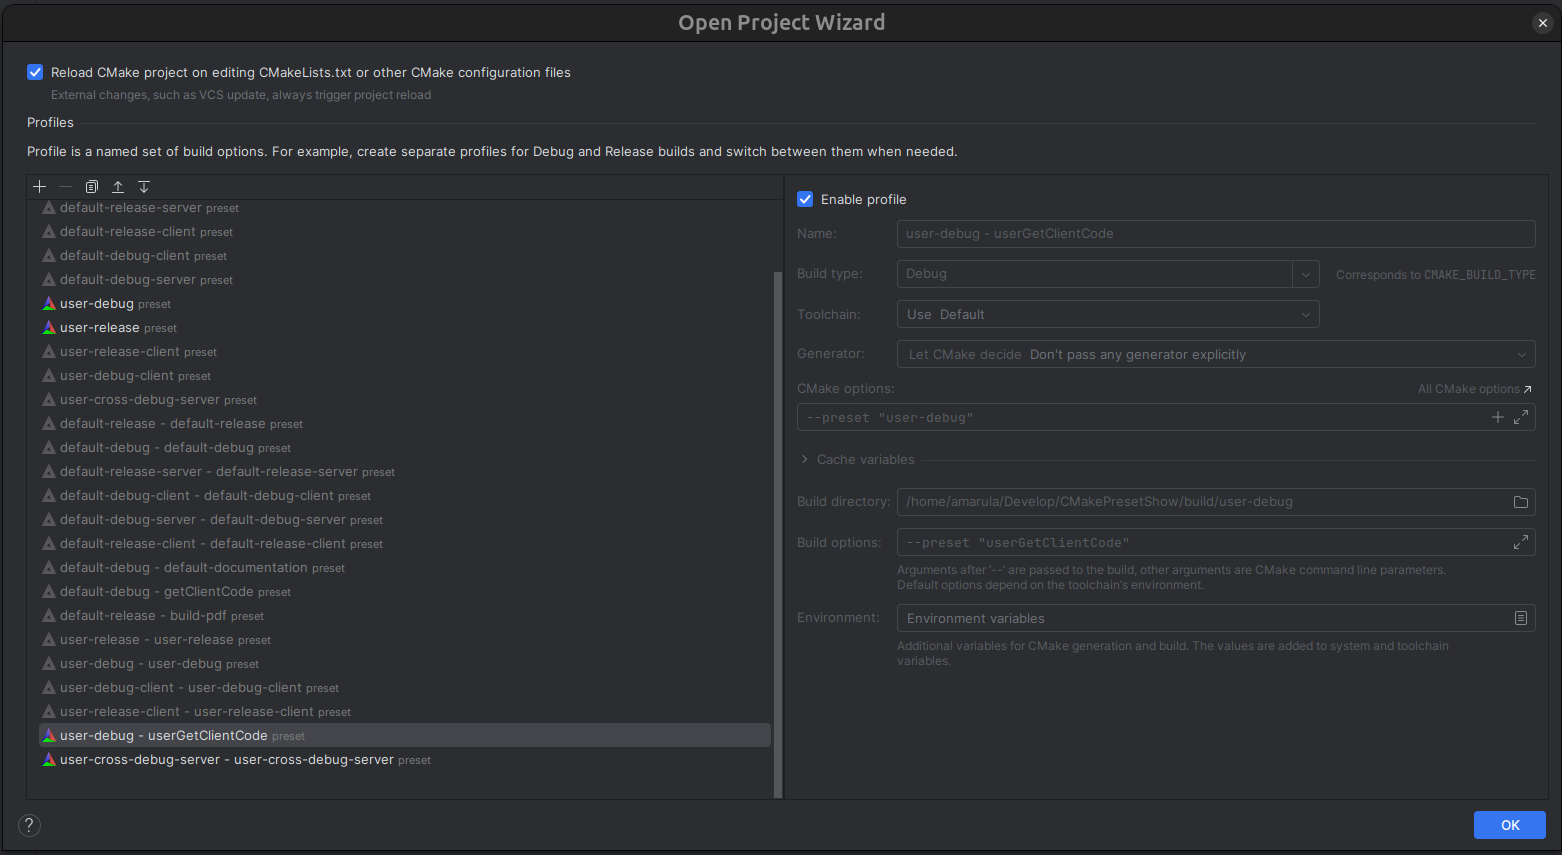
\includegraphics[height=6.5cm]{pictures/clion_show_presets.png}}
		\only<2>{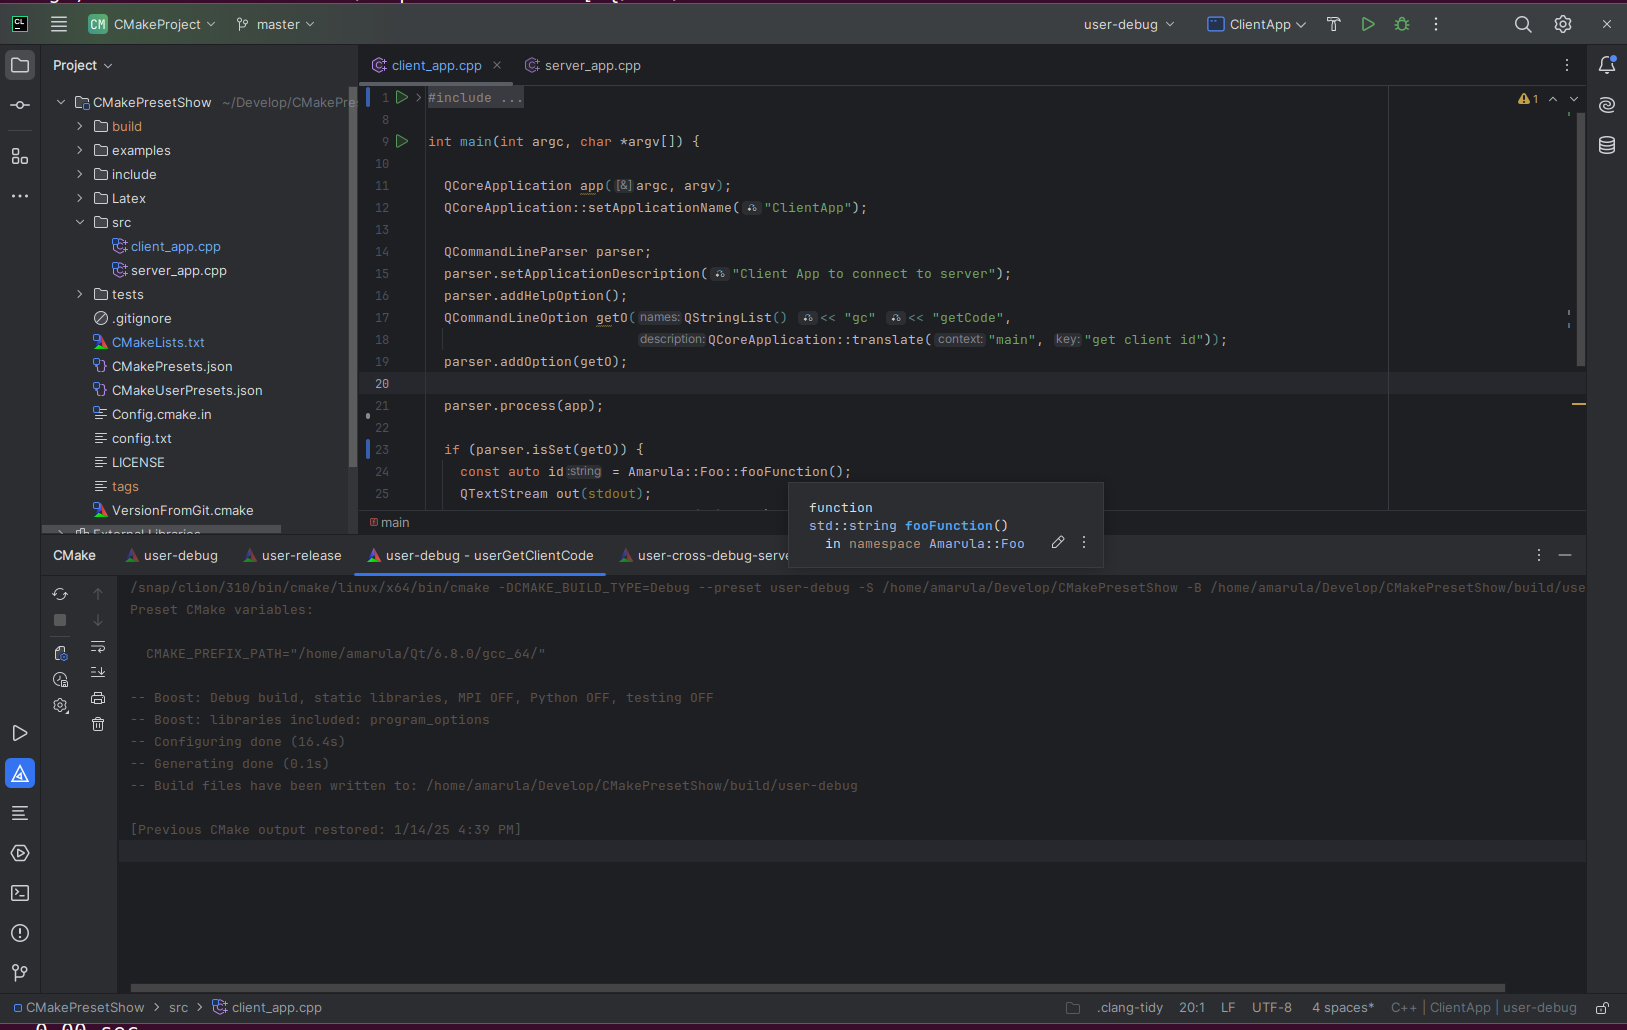
\includegraphics[height=6.5cm]{pictures/clion_show_presets_tabs.png}}
		\end{center}
\end{frame}
\begin{frame}[fragile]{IDEs: Qt Creator}\small%
	\vspace{2cm}
	\begin{center}
	\only<1>{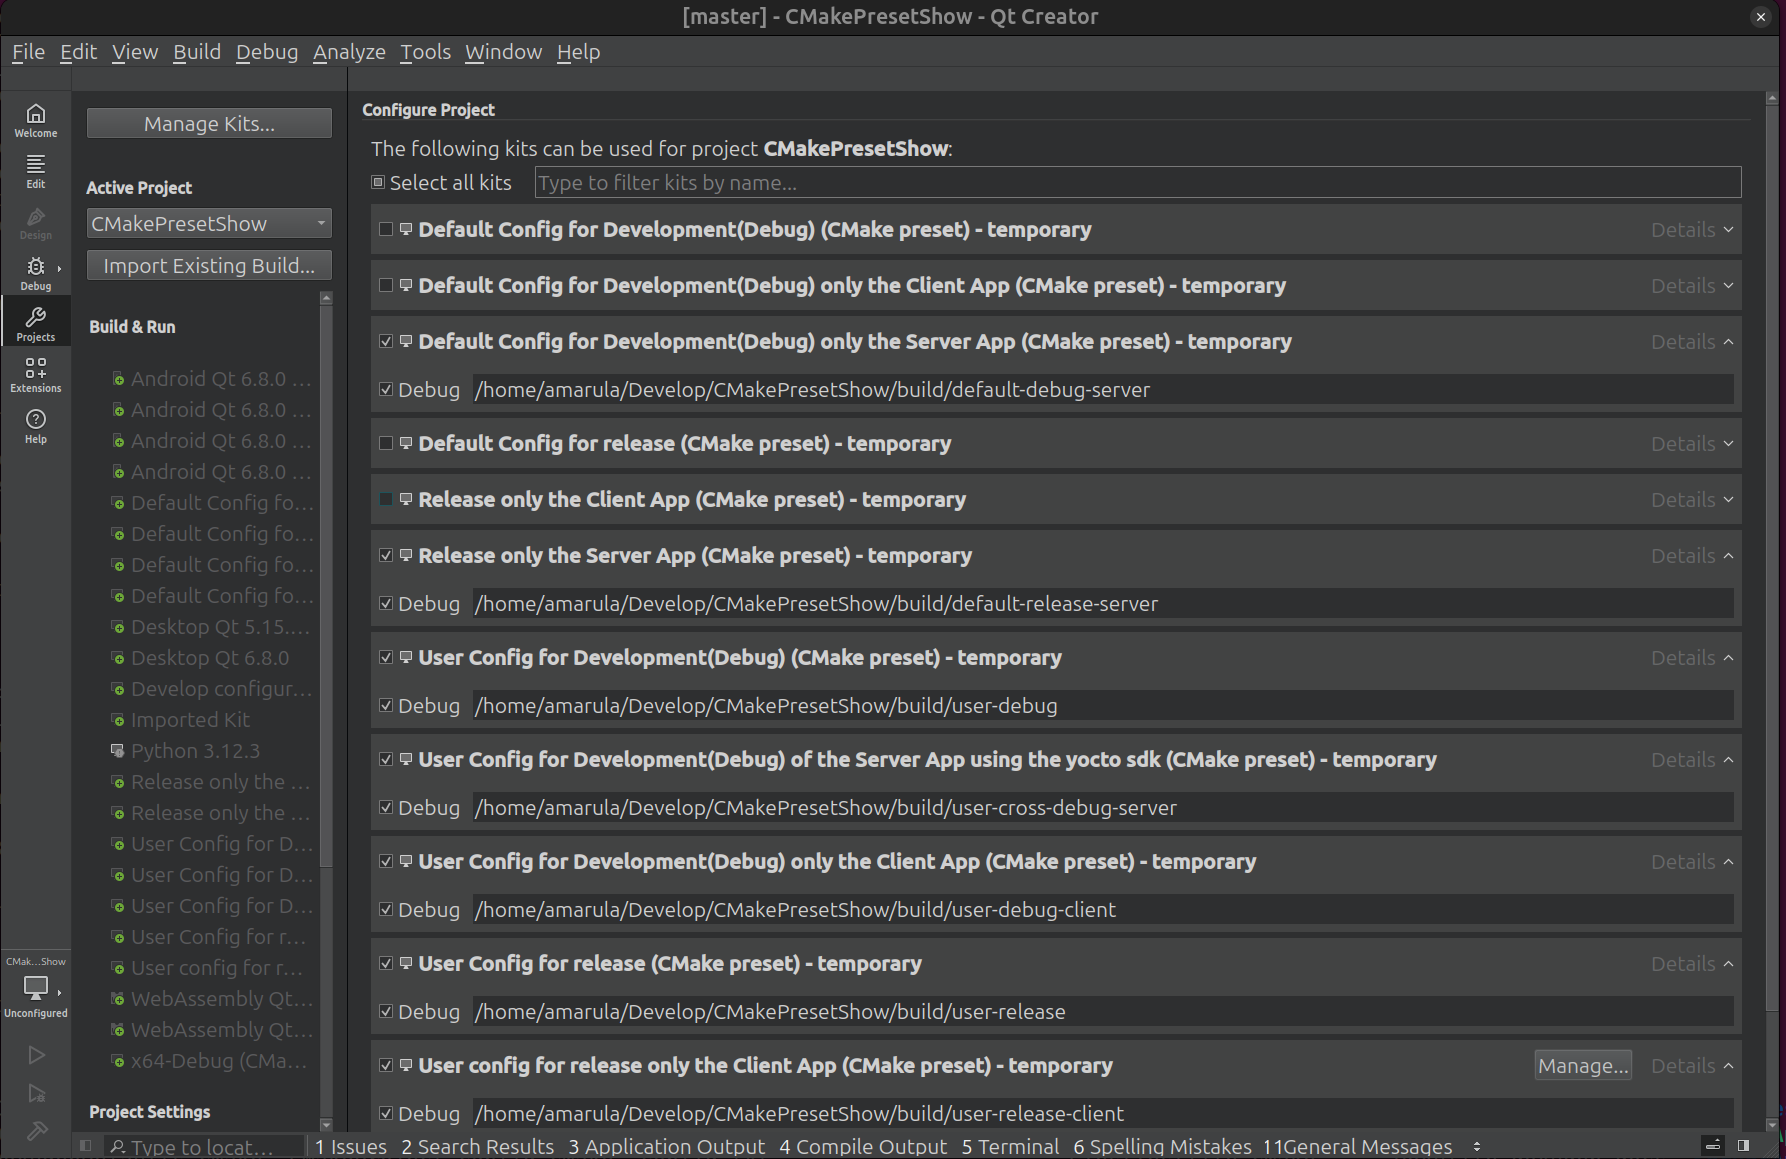
\includegraphics[height=7cm]{pictures/qtcreator_presets.png}}
	\only<2>{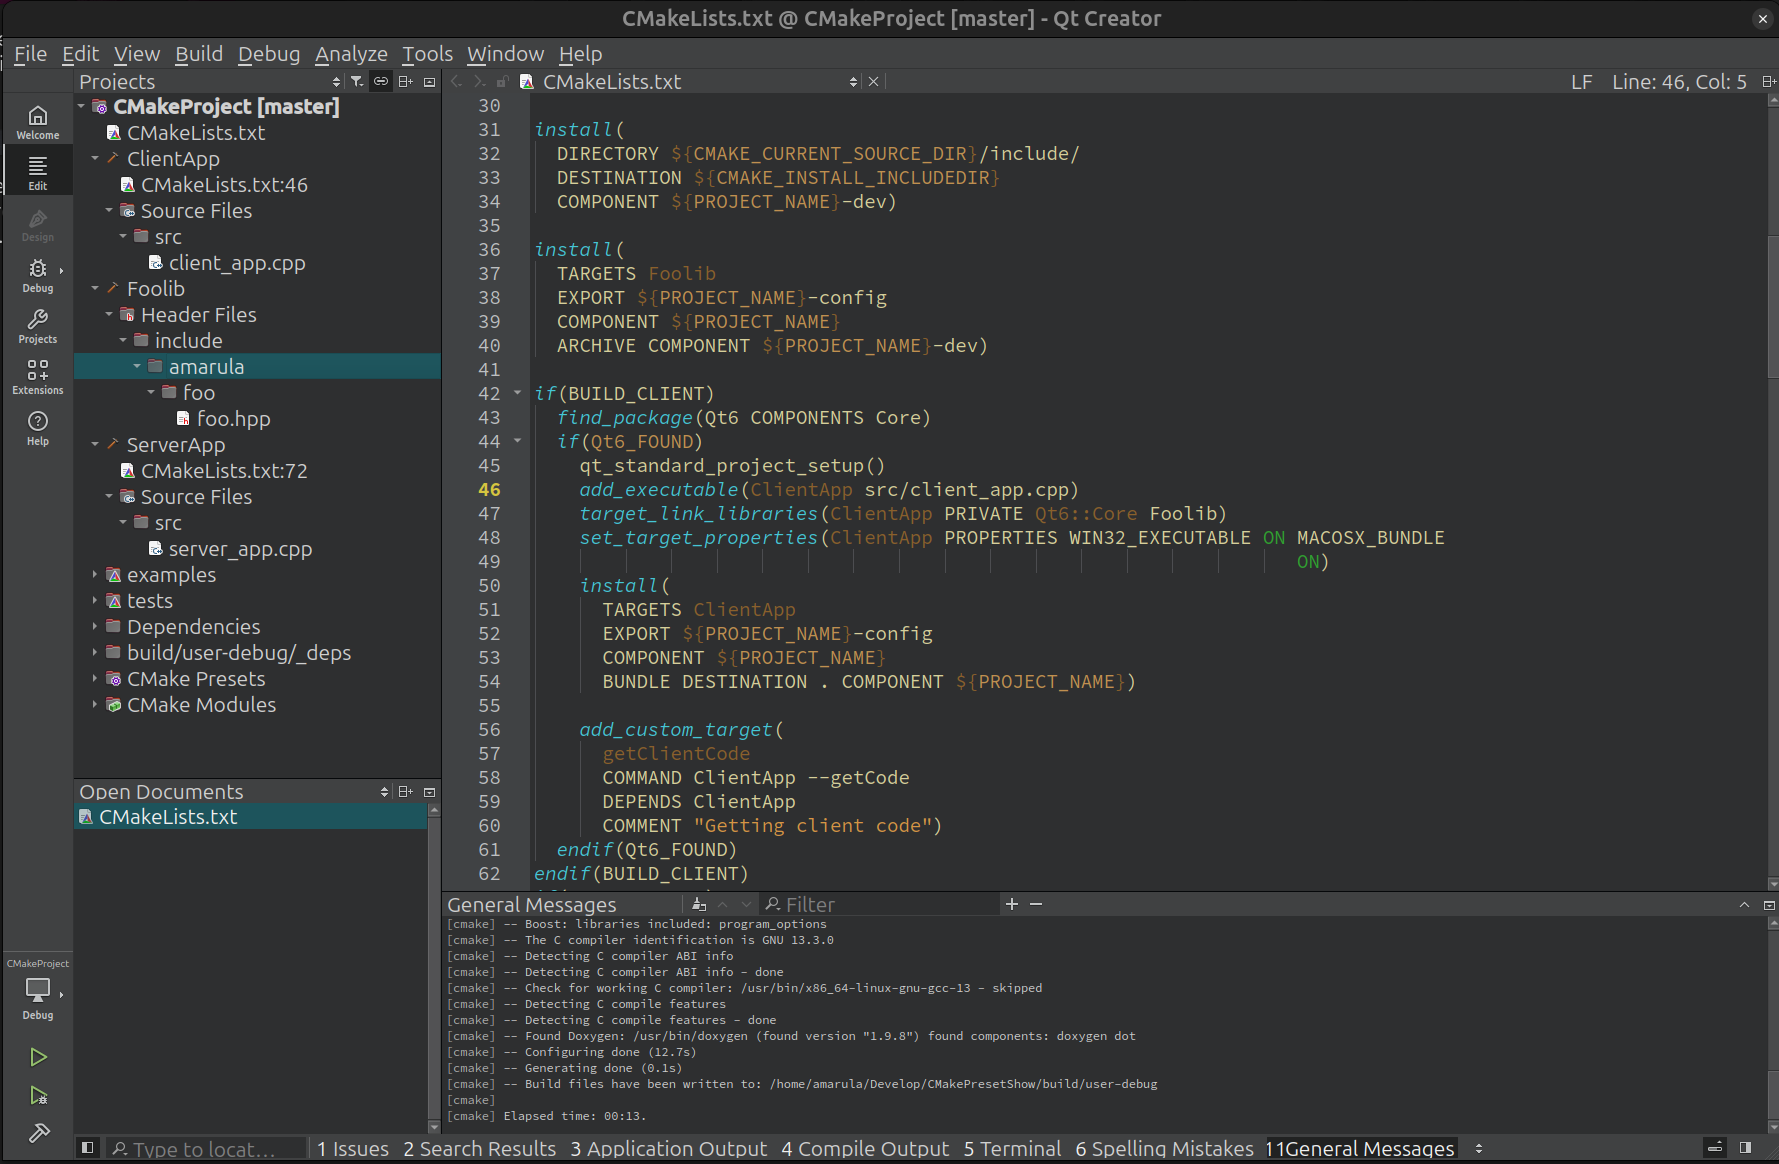
\includegraphics[height=7cm]{pictures/qtcreator_user_debug.png}}
	\only<3>{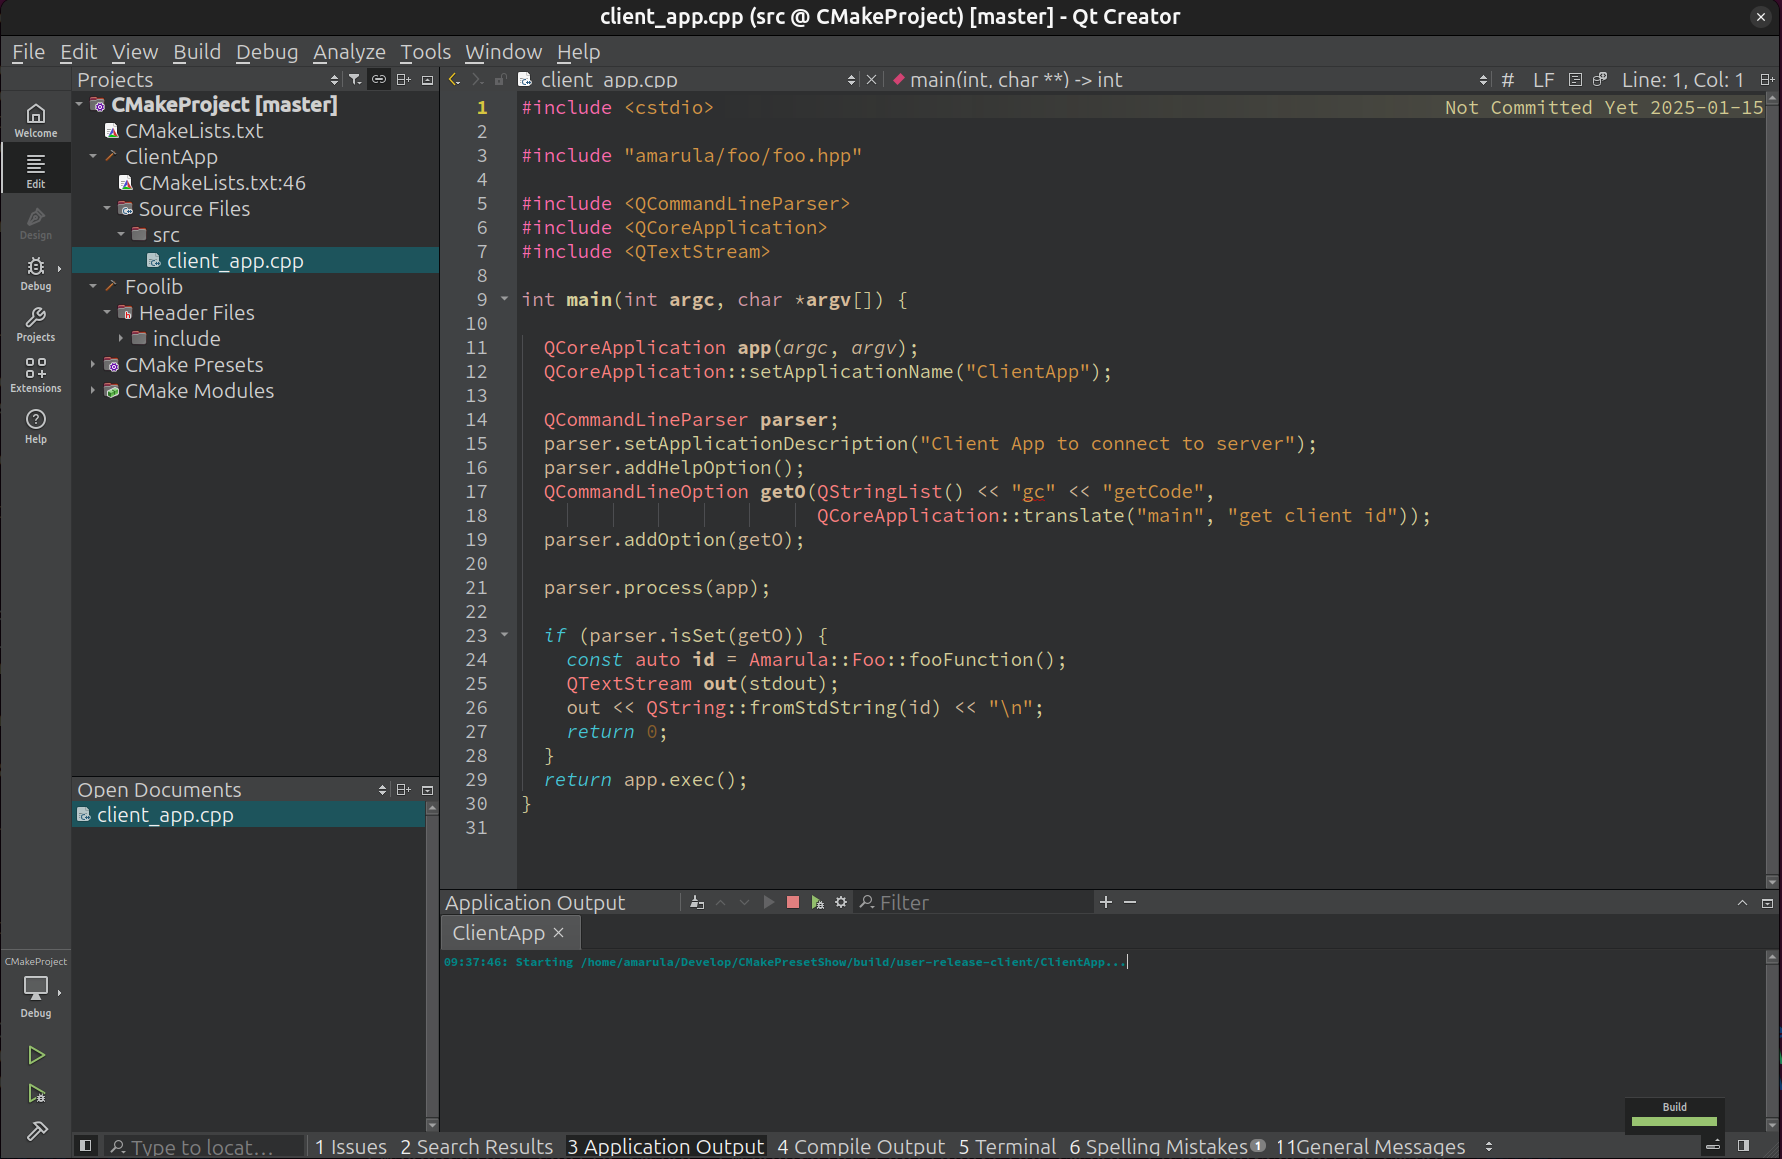
\includegraphics[height=7cm]{pictures/qtcreator_user_release_client.png}}
\end{center}
\end{frame}
\begin{frame}[fragile]{Continuous Integration}\small%
	\vspace{2cm}
	\begin{center}
		\lstinputlisting[firstline=27, lastline=50]{../.github/workflows/conf-build-test.yml}
	\end{center}
\end{frame}

\bigtemplate{Demo time}{
}

\begin{frame}[fragile]{Recommendations}\small%
			% This suggestion is found everywhere but many times is overlooked.
			% Well-defined targets will make your library/app easy to be reused
	\begin{itemize}
		\item Use CMake targets%
			\begin{columns}
				\column{0.5\textwidth}
				\begin{lstlisting}[language=sh]
pkg_check_modules(FOO REQUIRED foo)
				\end{lstlisting}%
				\column{0.5\textwidth}
				\begin{lstlisting}[language=sh]
add_subdirectory(foo)
FetchContent_MakeAvailable(foo)
find_package(foo CONFIG)
pkg_check_modules(FOO REQUIRED IMPORTED_TARGET foo)
				\end{lstlisting}%
			\end{columns}
			\begin{columns}
				\column{0.5\textwidth}  % First column takes 50% width
				\begin{lstlisting}[language=sh]
include_directories(${utils_INCLUDE_DIRS})
...
				\end{lstlisting}%
				\column{0.5\textwidth}  % Second column takes 50% width
				\begin{lstlisting}[language=sh]
target_include_directories(foo <INTERFACE|PUBLIC|PRIVATE> ${utils_INCLUDE_DIRS})
...
				\end{lstlisting}%
			\end{columns}
	\end{itemize}
\end{frame}

\begin{frame}[fragile]{Recommendations}\small%
	\vspace{1cm}
	\begin{itemize}
		\item Write/expose the minimum in each file/scope
	\end{itemize}
			\begin{columns}
				\column{0.5\textwidth}
				\begin{lstlisting}[language=sh]
#CMakeLists.txt
set(CMAKE_PREFIX_PATH /home/amarula/Qt/6.8.0/gcc_64/)
				\end{lstlisting}%
				\column{0.5\textwidth}
				\begin{lstlisting}[language=sh]
#CMakeUserPresets.json
"cacheVariables": {
	"CMAKE_PREFIX_PATH": "/home/amarula/Qt/6.8.0/gcc_64/"
}
				\end{lstlisting}%
			\end{columns}
			\begin{columns}
				\column{0.5\textwidth}
				\begin{lstlisting}[language=sh]
#CMakeLists.txt
set(CMAKE_BUILD_TYPE Debug)
				\end{lstlisting}%
				\column{0.5\textwidth}
				\begin{lstlisting}[language=sh]
#CMakePresets.json
"cacheVariables": {
	"CMAKE_BUILD_TYPE": "Debug"
}
				\end{lstlisting}%
			\end{columns}
			\begin{columns}
				\column{0.5\textwidth}
				\begin{lstlisting}[language=sh]
target_link_libraries(Foolib Qt6::Core)
target_link_libraries(Foolib Boost::program_options)
				\end{lstlisting}%
				\column{0.5\textwidth}
				\begin{lstlisting}[language=sh]
target_link_libraries(Foolib PUBLIC Qt6::Core)
target_link_libraries(Foolib PRIVATE Boost::program_options)
				\end{lstlisting}%
			\end{columns}
			\begin{columns}
				\column{0.5\textwidth}
				\begin{lstlisting}[language=sh]
find_dependency(Qt6 COMPONENTS Core)
find_dependency(Boost COMPONENTS program_options)
				\end{lstlisting}%
				\column{0.5\textwidth}
				\begin{lstlisting}[language=sh]
find_dependency(Qt6 COMPONENTS Core)
				\end{lstlisting}%
			\end{columns}
\end{frame}

\begin{frame}[fragile]{Recommendations}\small%
	\vspace{1cm}
	\begin{itemize}
		\item Choose well your \texttt{inherits}.
	\end{itemize}
\end{frame}
\bigtemplate{Conclusions}{
	\begin{itemize}
		\item Self-contained, reusable, and modularized CMake project
			\begin{itemize}
				\item Use CMake targets
				\item Export the targets and declare their dependencies
			\end{itemize}
		\item CMake Presets
			\begin{itemize}
				\item The final touch in creating a self-contained and reusable project
				\item Standard entry point when setting up a CMake/C++ project
			\end{itemize}
	\end{itemize}
}
\bigtemplate{Thank you for your attention}{

\begin{columns}
	\column{0.5\textwidth}			
	\textcolor{EDD_green}{Contact us:}
	\quad \qrcode{https://www.amarulasolutions.com/contact}

	\vspace{1cm}
	\tiny{\href{https://www.amarulasolutions.com/contact}{https://www.amarulasolutions.com/contact}}
	\column{0.5\textwidth}	
	\textcolor{EDD_green}{Download:}
	\quad \qrcode{https://github.com/EddyTheCo/CMakePresetsShow}

	\vspace{1cm}
	\tiny{\href{https://github.com/EddyTheCo/CMakePresetsShow}{https://github.com/EddyTheCo/CMakePresetsShow}}
\end{columns}
			
		}
\begin{frame}[allowframebreaks] {References}
	\bibliographystyle{apalike}\vspace{1cm}
	\scriptsize        \begin{spacing}{0.5}  \fontdimen2\font=0.4ex
	\bibliography{biblio.bib}\end{spacing}
\end{frame}

\end{document}
